\documentclass[10pt]{article}
\usepackage[top=1in, bottom=1.2in]{geometry}
\linespread{1} % line spacing
\geometry{letterpaper}
\usepackage{tabularx}
\usepackage[parfill]{parskip} % begin paragraphs with an empty line rather than an indent
\usepackage[ocgcolorlinks]{hyperref} %ocg coverts links to black when you print -- downside of unbreakable lines



% New command \CustomLabel{labelname} creates a hypertarget and label for referencing
\makeatletter
 \newcommand{\CustomLabel}[1]{\Hy@raisedlink{\hypertarget{#1}{}}\label{#1}}
\makeatother

% Graph Stuff
\usepackage{tikz}
\usetikzlibrary{trees} % this is to allow the fork right path
\usetikzlibrary{calc} % for hyperlinking nodes

\usetikzlibrary{positioning}

% Styling for Graphs
\tikzset{
    basic/.style  = {thin, draw, text width=5em, font=\sffamily, rectangle, minimum size=2em, align=center},
    root/.style   = {basic},
    edge from parent fork down,
        level 2/.style = {basic, grow=down, edge from parent path={(\tikzparentnode.south) |- (\tikzchildnode.west)}},
        level 3/.style = {basic, xshift=1ex,anchor=west},
            subA/.style={level distance=6ex},
            subB/.style={level distance=12ex},
            subC/.style={level distance=18ex},
    hyperlink node/.style={
      postaction={
        path picture={
          \path let
          \p1 = (path picture bounding box.south west),
          \p2 = (path picture bounding box.north east),
          \p3 = (\x2-\x1,\y2-\y1)
          in
          (path picture bounding box.center)
          node[inner sep=0pt,anchor=center,outer sep=0pt]
          {\hyperlink{#1}{\phantom{\rule{\x3}{\y3}}}};
        }
      },
    }
}

\title{\bf Checkers Design Document}
\author{2me3}
\date{}

\begin{document} %%%%%%%%%%%%%%%%%%%%%%%%%%%%%%%%%%%%%%%%%%%%%%%%%%%%%%%%%%%%%%%%%%%%%%%%%%
\maketitle

\tableofcontents

\section{Introduction}
    This document contains the decomposition, uses relationship, and traceability.
    Note: Red links and the Uses diagram are clickable hyperlinks (depending on your PDF reader).
    
\section{Module Guide}

\subsection{Hardware Hiding Module}
\iffalse
    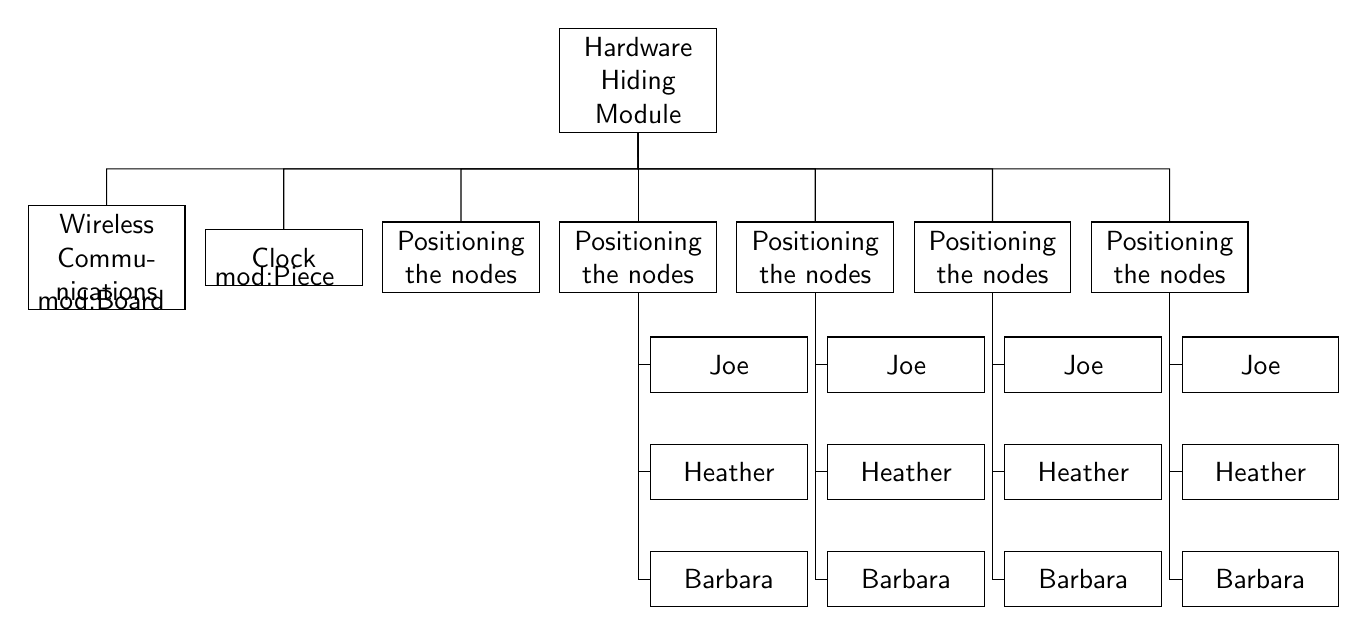
\begin{tikzpicture}[scale=1.5, align=center]
        \node[root] {Hardware Hiding Module}
        child {node[level 2, hyperlink node=mod:Board]{Wireless Communications}}
        child {node[level 2, hyperlink node=mod:Piece]{Clock}}
        child {node[level 2]{Positioning the nodes}}
        child {node[level 2]{Positioning the nodes}
            child[subA] {node[level 3]{Joe}}
            child[subB] {node[level 3]{Heather}}
            child[subC] {node[level 3]{Barbara}}}
        child {node[level 2]{Positioning the nodes}
            child[subA] {node[level 3]{Joe}}
            child[subB] {node[level 3]{Heather}}
            child[subC] {node[level 3]{Barbara}}}
        child {node[level 2]{Positioning the nodes}
            child[subA] {node[level 3]{Joe}}
            child[subB] {node[level 3]{Heather}}
            child[subC] {node[level 3]{Barbara}}}
        child {node[level 2]{Positioning the nodes}
            child[subA] {node[level 3]{Joe}}
            child[subB] {node[level 3]{Heather}}
            child[subC] {node[level 3]{Barbara}}}
        ;
    \end{tikzpicture}
\fi
    
    \subsubsection{Input Module}\CustomLabel{mod:Input}
    \begin{tabularx}{\linewidth}{ >{\bfseries}r X }
        Type            & Hardware Module \\
        Secret          & This module translate mouse clicks and keyboard presses to be used by the rest of the software. \\
        Responsibilites & This module will take mouse and keyboard input and convert it to software usable states. \\
        Uses            & None \\
        Design          & \ref{mis:Input} \\
        Code File       & Inside Game1.cs, and built into C\#. \\
        Explanation     & The input module is a hardware hiding module since it translates hardware inputs to software. \\
    \end{tabularx}

\subsection{Behaviour Hiding Module}

    \subsubsection{Piece Module}\CustomLabel{mod:Piece}
        \begin{tabularx}{\linewidth}{ >{\bfseries}r X }
            Type            & Software Module \\
            Secret          & This module hides and separates specific piece information. \\
            Responsibilites & This will hold the necessary components to describe what a game piece will contain, which will be seperate from the game board. \\
            Uses            & None \\
            Design          & \ref{mis:Piece} \\
            Code File       & Piece.cs \\
            Explanation     & The piece is a part of behaviour hiding since the piece module holds specific piece information and outputs values needed by other modules. \\
        \end{tabularx}

\subsection{Software Decision Hiding Module}

    \subsubsection{Board Module}\CustomLabel{mod:Board}
        \begin{tabularx}{\linewidth}{ >{\bfseries}r X }
            Type            & Software Module \\
            Secret          & This module serves to hide the secret of how the board is defined internally. \\
            Responsibilites & This module is responsible for holding the necessary components and attributes to setup the board and describe piece locations. \\
            Uses            & \ref{mod:Piece} \\
            Design          & \ref{mis:Board} \\
            Code File       & Board.cs \\
            Explanation     & The board is a part of software decision hiding since the board implements a data structure that holds the placement of the pieces, this data structure might be changed for increased performance. Another software decision is deciding how to take user input to parse the placement of pieces. \\
        \end{tabularx}

    \subsubsection{Game1 Module}\CustomLabel{mod:Game1}
        \begin{tabularx}{\linewidth}{ >{\bfseries}r X }
            Type            & Software Module \\
            Secret          & This module hides how the graphics are displayed and how we switch between states of the game. \\
            Responsibilites & This module will be the responsible for the initial execution of the game, this class connects and launches critical components together. \\
            Uses            & \ref{mod:Board}, \ref{mod:Piece}, \ref{mod:Input} \\
            Design          & \ref{mis:Game1} \\
            Code File       & Game1.cs \\
            Explanation     & The module is a part of software decision hiding since it determines how we draw the graphics and what to do when we switch between states of the game. \\
        \end{tabularx}
        
        
        
        \section{Uses Relationship} 
\tikzset{main node/.style={rectangle,fill=blue!5,draw,minimum size=1cm,inner sep=0pt},
}
  \begin{tikzpicture}
    \node[main node, hyperlink node = mod:Game1] (1) {Game1};
    \node[main node, hyperlink node = mod:Board] (2) [below left = 2.3cm and 1.5cm of 1]  {Board};
    \node[main node, hyperlink node = mod:Piece] (3) [below left = 2.3cm and 1cm of 2] {Piece};
    \node[main node, hyperlink node = mod:Input] (4) [below right = 2.3cm and 1.5cm of 1] {Input};

    \path[draw,thick,->]
    (1) edge node {} (2)    % game1 to board
    (2) edge node {} (3)    % board to piece
    (1) edge node {} (4);   % game1 to input
    %%
    
    \iffalse % this is just here in case we add more modules that aren't connected to anything
    \begin{scope}[xshift=4cm]
    \node[main node] (1) {$1$};
    \node[main node] (2) [right = 2cm  of 1]  {$2$};
    \node[main node] (3) [below = 2cm  of 1] {$3$};
    \node[main node] (4) [right = 2cm  of 3] {$4$};

    \path[draw,thick]
    (1) edge node {} (2)
    (1) edge node {} (4)
    (3) edge node {} (2)
    (3) edge node {} (4)
    ;
    \end{scope}
    \fi
\end{tikzpicture}


\newpage
%%%%%%%%%%%%%%%%%%%%%%%%%%%%%%%%%%%%%%%%%%%%%%%%%%%%%%%%%%%%%%%%%%%%%%%%%%%%%%%%%%%%%%%%%%%%%%%%%%%%%%



\section{Module Design (MIS and MID)}


       
    \subsection{Piece Module}\CustomLabel{mis:Piece}
    \subsubsection{Interface}
        \begin{tabularx}{\linewidth}{@{} >{\bfseries}r Xp{5cm} }
            Types           & \begin{tabular}[t]{@{} l p{8cm}} 
                                     & \\
                                    typeState & enumerate if the piece is normal or king \\
                                    player & enumerate if piece owned by Black or White \\
                              \end{tabular} \\
                              
            Constants       & \begin{tabular}[t]{@{} l p{8cm}} 
                                     & \\
                                    None & \\
                              \end{tabular} \\

            Access Programs & \begin{tabular}[t]{@{} l p{8cm}}
                                     & \\
                                    getType() : typeState & Retrieves the piece's current type. \\
                                    setType(newType : typeState) & Changes the piece's type. \\ 
                                    getOwner() : player & Says who owns the piece. \\
                              \end{tabular}
        \end{tabularx}
        
    \subsubsection{Implementation}
        \begin{tabularx}{\linewidth}{ >{\bfseries}r Xp{5cm} }
            Variables       & \begin{tabular}[t]{@{} l p{8cm}} 
                                     & \\
                                    pieceType : typeState & holds current piece type \\
                                    owner : player & holds information of the piece's owner \\
                              \end{tabular} \\

            Access Programs & \begin{tabular}[t]{@{} l l p{8cm}} 
                                     & \\
                                    \bf{getType()} : typeState & \\
                                    Inputs &  None \\
                                    Updates & None \\
                                    Outputs & pieceType \\
                                    Description & WHAT DO? \\
                                     & \\
                                    \bf{setType(newType : typeState)} & \\
                                    Inputs & newType \\
                                    Updates & None \\ 
                                    Outputs & pieceType \\
                                    Description & WHAT DO? \\
                                     & \\
                                    \bf{getOwner()} : player & \\
                                    Inputs & None \\
                                    Updates & None \\
                                    Outputs & owner \\ 
                                    Description & WHAT DO? \\
                              \end{tabular} \\
                              
        \end{tabularx}
        
        
        
        
        
    \subsection{Board Module}\CustomLabel{mis:Board}
    \subsubsection{Interface}
        \begin{tabularx}{\linewidth}{@{} >{\bfseries}r Xp{5cm} }
            Types           & \begin{tabular}[t]{@{} l p{8cm}} 
                                     & \\
                                    None & \\
                              \end{tabular} \\
                              
            Constants       & \begin{tabular}[t]{@{} l p{8cm}} 
                                     & \\
                                    None & \\
                              \end{tabular} \\

            Access Programs & \begin{tabular}[t]{@{} p{4cm} p{8cm}}
                                     & \\
                                    setUpBoard() & Sets up board based on user input. \\
                                     & \\
                                    getPiece(col : int, row : int) : Piece & This method is used to determine if a piece exists on a square of the board. If the piece does exist, we pass it along to the caller. \\ 
                                     & \\
                                    placePiece(col : int, row : int, piece : Piece) & Places the piece on the board while checking if the placement is legal (in terms of checkers). \\
                                     & \\
                                    movePiece(fromCol : int, fromRow : int, toCol : int, toRow : int) & Moves the piece from starting to end positions while checking if the movement is valid (in terms of checkers). \\
                                     & \\
                                    clear() & Removes all pieces from the board. \\
                                     & \\
                             \end{tabular}
        \end{tabularx}
        
    \subsubsection{Implementation}
        \begin{tabularx}{\linewidth}{ >{\bfseries}r Xp{2cm} }
            Types           & \begin{tabular}[t]{@{} l p{8cm}} 
                                 & \\
                                None & \\
                                \end{tabular} \\
            Constants       & \begin{tabular}[t]{@{} l p{8cm}} 
                                 & \\
                                None & \\
                            \end{tabular} \\
            Variables       & \begin{tabular}[t]{@{} l p{8cm}} 
                                     & \\
                                    pieceArray : array & Contains all the Piece objects currently on the board in an array. \\
                                    numWhitePieces : int & Holds the number of white pieces on the board as an integer. \\
                                    numBlackPieces : int & Holds the number of black pieces on the board as an integer. \\
                              \end{tabular} \\
            Access Programs & \\
                            & \bf{setUpBoard(input : string)} \\
                            & \begin{tabular}[t]{@{} p{2.5cm} p{10cm}} 
                                    Inputs & input \\
                                    Outputs & pieceArray, numWhitePieces, numBlackPieces \\
                                    Updates & None \\
                                    Description & Parses input to be interpreted as Piece locations. Place Piece on correct Piece location using the PlacePiece() access program. numWhitePieces' = numWhitePieces + c and numBlackPieces' = numBlackPieces + d where c and d are between 0 and 12. pieceArray' = pieceArray with c + d more PieceObjects.\\
                                     & \\
                                     \end{tabular} \\
                            & \bf{getPiece(col : int, row : int)} : Piece \\
                            & \begin{tabular}[t]{@{} p{2.5cm} p{10cm}} 
                                    Inputs & col, row \\
                                    Outputs & piece \\
                                    Updates & None \\ 
                                     & \\
                                     \end{tabular} \\
                            & \bf{placePiece(col : int, row : int, piece : Piece)} \\
                            & \begin{tabular}[t]{@{} p{2.5cm} p{10cm}}
                                    Inputs &  col, row, piece \\
                                    Outputs & None \\
                                    Updates & pieceArray, numWhitePieces, numBlackPieces \\ 
                                    Description & If piece placement is valid, it will put it there in the data structure. Either numWhitePieces' = numWhitePieces + 1 or numBlackPieces' = numWhitePieces + 1. pieceArray' = pieceArray with one more Piece object.\\
                                     & \\
                                     \end{tabular} \\
                            & \bf{movePiece(fromCol : int, fromRow : int, toCol : int, toRow : int)} \\
                            & \begin{tabular}[t]{@{} p{2.5cm} p{10cm}}
                                    Inputs  & None \\
                                    Outputs & None \\
                                    Updates & None \\
                                     & \\
                                     \end{tabular} \\
                            & \bf{clear()} & \\
                            & \begin{tabular}[t]{@{} p{2.5cm} p{10cm}}
                                    Inputs  & None \\
                                    Outputs & pieceArray, numWhitePieces, numBlackPieces \\
                                    Updates & None \\
                                    Description & pieceArray' = Array of null objects, numWhitePieces' = 0 or numBlackPieces' = 0. \\
                                     \end{tabular} \\
        \end{tabularx}
        


        
        
        
        
    \subsection{Game1 Module}\CustomLabel{mis:Game1}
    \subsubsection{Interface}
        \begin{tabularx}{\linewidth}{@{} >{\bfseries}r Xp{5cm} }
            Types           & \begin{tabular}[t]{@{} l p{8cm}} 
                                     & \\
                                    state & enumerate if the game is in Menu, Setup, or Playing \\
                              \end{tabular} \\
                              
            Constants       & \begin{tabular}[t]{@{} l p{8cm}} 
                                     & \\
                                    None & \\
                              \end{tabular} \\

            Access Programs & \begin{tabular}[t]{@{} l p{8cm}}
                                     & \\
                                    Update() & Allows the game to run logic such as switching state, updating the game, and gathering input. \\
                                    Draw() & Draws the correct graphics on screen depending on the state. \\ 
                                    takeInput() & Takes user input for setting up a board. \\
                              \end{tabular}
        \end{tabularx}
        
    \subsubsection{Implementation}
        \begin{tabularx}{\linewidth}{ >{\bfseries}r Xp{5cm} }
            Variables       & \begin{tabular}[t]{@{} l p{8cm}} 
                                     & \\
                                    currentState : state & holds information of the current state \\
                                    input : string & holds board setup from user \\ 
                                    board : Board & \\
                                    pieceList : List &  Holds information of where to graphically place each piece. \\
                                    
                              \end{tabular} \\

            Access Programs & \begin{tabular}[t]{@{} l p{8cm}} 
                                     & \\
                                    \bf{Update()} & \\
                                    Inputs &  None \\
                                    Updates & currentState \\
                                    Outputs & None \\
                                    Description & Changes the state based on keyboard press or mouse presses on graphical buttons.\\
                                     & \\
                                    \bf{Draw()} & \\
                                    Inputs & board \\
                                    Updates & pieceList \\
                                    Outputs & None \\
                                    Description & Draws the buttons, board tiles and pieces in proper place on the screen. The piece locations are stored in pieceList. And we just loop through the graphics objects to draw them each frame. \\
                                     & \\
                                    \bf{takeInput()} & \\
                                    Inputs & input \\
                                    Updates & None \\
                                    Outputs & board \\ 
                                    Description & Takes user input and sends it to the board using board.SetUpBoard().\\
                              \end{tabular} \\
                              
        \end{tabularx}


    \subsection{Input Module}\CustomLabel{mis:Input}
    \subsubsection{Interface}
        \begin{tabularx}{\linewidth}{@{} >{\bfseries}r Xp{5cm} }
            Types           & \begin{tabular}[t]{@{} l p{8cm}} 
                                     & \\
                                    Mouse & enumeration of mouse button states \\
                                    Keys & enumerates keyboard buttons \\
                              \end{tabular} \\
                              
            Constants       & \begin{tabular}[t]{@{} l p{8cm}} 
                                     & \\
                                    None & \\
                              \end{tabular} \\

            Access Programs & \begin{tabular}[t]{@{} l p{8cm}}
                                     & \\
                                    GetState() : Mouse & Gets if mouse button is pressed. \\
                                    IsKeyDown(key : Keys) : bool & Checks if the key is pressed. \\
                              \end{tabular}
        \end{tabularx}
        
    \subsubsection{Implementation}
        \begin{tabularx}{\linewidth}{ >{\bfseries}r Xp{5cm} }
            Variables       & \begin{tabular}[t]{@{} l p{8cm}} 
                                     & \\
                                    mouseState : Mouse & Holds if mouse is pressed. \\
                                    mouseClickedPiece & Holds the graphical object the mouse is clicking on. \\
                                    mousePos & Stores current mouse position. \\
                              \end{tabular} \\

            Access Programs & \begin{tabular}[t]{@{} l p{8cm}} 
                                     & \\
                                    \bf{GetState()} & \\
                                    Inputs &  None \\
                                    Updates & None \\
                                    Outputs & mouseState \\
                                     & \\
                                    \bf{IsKeyDown(key : Keys)} & \\
                                    Inputs & None \\
                                    Updates & None \\
                                    Outputs & None \\ 
                              \end{tabular} \\
                              
        \end{tabularx}
        
        
        
        
        
        
        
        
        

\end{document}












